\documentclass{beamer}

\usepackage{default}
\usepackage[german]{babel}
\usepackage[utf8]{inputenc}                   % replace by the encoding you are using

\usetheme{Berlin}

%Header Settings
%\setbeamertemplate{headline}{}

%Footer Settings
\setbeamertemplate{navigation symbols}{
	\usebeamerfont{footline}%
	\usebeamercolor[fg]{footline}%
	\hspace{1em}%
	\insertframenumber/\inserttotalframenumber
}

\title[Java]{Java}
\author[W. Bombardelli]{William Bombardelli}
\institute[Schweizerschule Mexiko]
{
	\vskip 12pt
	Schweizerschule Mexiko, Ciudad de México, Mexiko \\
	\texttt{E-Mail...}
}
\date{4. September 2019}

\makeatletter
\hypersetup{
	pdftitle = {\@title}, pdfkeywords = {Java}, pdfauthor = {\@author}
} 
\makeatother

\begin{document}
	\begin{frame}
		\titlepage
	\end{frame}
	
	\begin{frame}
		\frametitle{Gliederung}
		\tableofcontents
	\end{frame}
	
	%-------------------
	% Organisation
	%-------------------
	\section{Organisation}
	\begin{frame}
		\frametitle{Organisation}
		
		\begin{itemize}
			\item Kurs: Java
			\begin{itemize}
				\item Einführung in die Programmierung mit Java
			\end{itemize}
			\item Lehrer: William Bombardelli
			\item Tempo: 2 Stunden pro Woche. Mittwoch 14.35
			\item Prüfungen: 1 Prüfung + 2 Aufgaben pro Semester
			\item Ziele:
			\begin{itemize}
				\item Probleme anhand eines Rechners lösen
				\item Programmen auf Java lesen bzw. verstehen und schreiben 
			\end{itemize}
			\item Literatur: 
			\begin{itemize}
				\item Oracle Java Tutorial: \url{https://docs.oracle.com/javase/tutorial}
				\item W3C Java Tutorial: \url{https://www.w3schools.com/java}
			\end{itemize}
		\end{itemize}
	\end{frame}

	%-------------------
	% Grundlagen
	%-------------------
	\section{Grundlagen}
	\begin{frame}
		\frametitle{Grundlagen}
		\tableofcontents[currentsection, currentsubsection] 
	\end{frame}

	\begin{frame}
		\frametitle{Algorithmus}
		\begin{itemize}
			\item Wie löst man ein Problem?
			\begin{itemize}
				\item Man definiert eine Methode/ Strategie. D.h. ein Algorithmus
				\item z.B. Eine endliche Sequenz von Einzelschritten
			\end{itemize} 
			\pause
			\vspace{10pt}
			\item Beispiel: Einen Schokokuchen zubereiten
			\pause
			\vspace{10pt}
			\item Algorithmus: Schokokuchen-Rezept
			\begin{enumerate}
				\item Form einfetten
				\item Backofen auf 180 Grad vorheizen
				\item Butter mit Zucker und Salz schlagen
				\item Eier zugeben
				\item ...
				\item 40 Min. backen
				\item Schokolade über den Kuchen gießen
				\item 30 Min. anziehen lassen
			\end{enumerate}
		\end{itemize}
	\end{frame}

	\begin{frame}
		\frametitle{Algorithmus - Beispiel}
		\centering 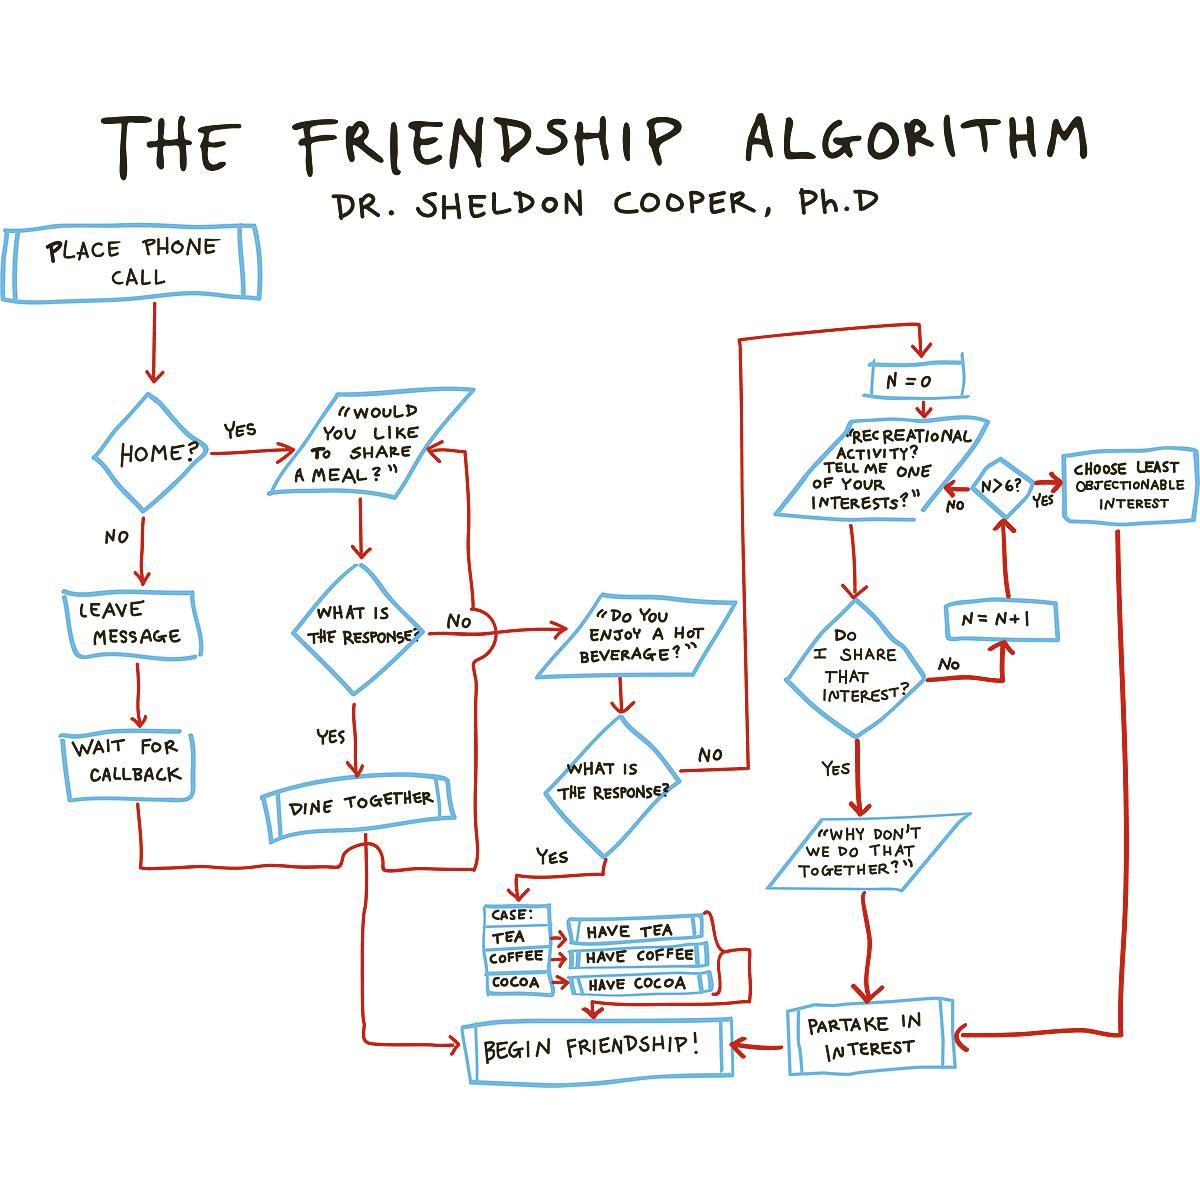
\includegraphics[height=.9\textheight]{Algorithmus}
	\end{frame}

	\begin{frame}
		\frametitle{Algorithmus - Beispiele}
		\pause
		\begin{itemize}
			\item Glühbirne wechseln
			\item Wäsche waschen
			\pause
			\vspace{10pt}
			\item schriftliche Division ($351 : 4 = 87\ Rest\ 3$)
			\item Multiplikation (verschiedene Algorithmen)
			\item lineare Gleichungen lösen ($ax = b$)
			\item Wurzeln für ein Polynom zweiten Grades finden ($ax^2 + bx + c$)
			\pause
			\vspace{10pt}
			\item Laufen
			\item Gesicht anerkennen
			\item ...
		\end{itemize}
	\end{frame}

	\begin{frame}
		\frametitle{Algorithmus - Glühbirne Wechseln}
		
	\end{frame}

	\begin{frame}
		\frametitle{Algorithmus - Nullstellen eines Polynoms zweiten Grades}
		\begin{itemize}
			\item Beispiel: Lösungen für ein Polynom mit Grad 2
			\item $P(x) = ax^2 + bx + c$
			\pause
			\vspace{10pt}
			\item Algorithmus:
			\begin{enumerate}
				\item Berechne $\Delta = b^2 - 4ac$
				\item Wenn $\Delta \ge 0$ dann
				\begin{enumerate}
					\item Berechne $x_1 = \frac{-b + \sqrt{\Delta}}{2a}$
					\item Berechne $x_2 = \frac{-b - \sqrt{\Delta}}{2a}$
					\item Lösung ist $x_1$ und $x_2$
				\end{enumerate}
				\item Sonst
				\begin{enumerate}
					\item keine reelle Lösung
				\end{enumerate}
			\end{enumerate}
		\end{itemize}
	\end{frame}

	\begin{frame}
		\frametitle{Programm}
		\begin{itemize}
			\item Ein Programm ist eine Implementierung eines Algorithmus auf einer Programmiersprache.
			\begin{itemize}
				\item z.B. Java, C, Python, ...
			\end{itemize}
			\item Ein Programm lässt sich von einem Rechner ausführen
			\item Programmieren heißt einem Rechner sagen, was er tun soll
		\end{itemize}
	\end{frame}

	\begin{frame}
		\frametitle{Programm - Beispiel in Java}
		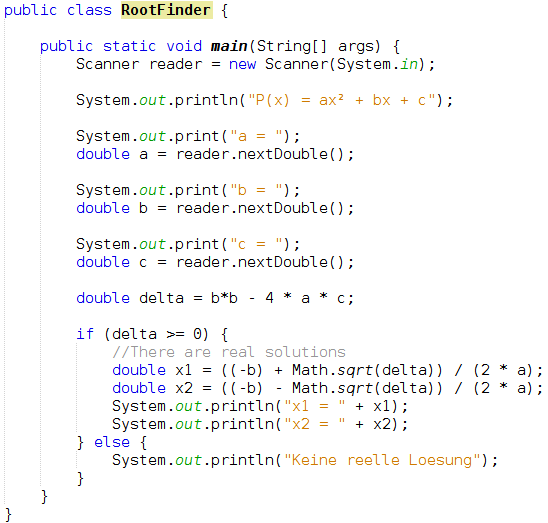
\includegraphics[height=.8\textheight]{Nullstellen-Java}
	\end{frame}

	\begin{frame}
		\frametitle{Programm - Vor- und Nachteile}
		\begin{itemize}
			\item {\color{green} schnell auszuführen}
			\item {\color{red} langsam zu lesen/ verstehen}
			\pause
			\vspace{10pt}
			\item {\color{green} automatisiert}
			\item {\color{green} wohldefiniert/ eindeutig}
			\item {\color{green} skalierbar - große Menge Daten}
			\pause
			\vspace{10pt}
			\item {\color{red} strikte Sprachen}
			\item {\color{red} viel zu detailliert}
		\end{itemize}
	\end{frame}

	\begin{frame}
		\frametitle{Problem - Algorithmus - Programm - Berechnung}
		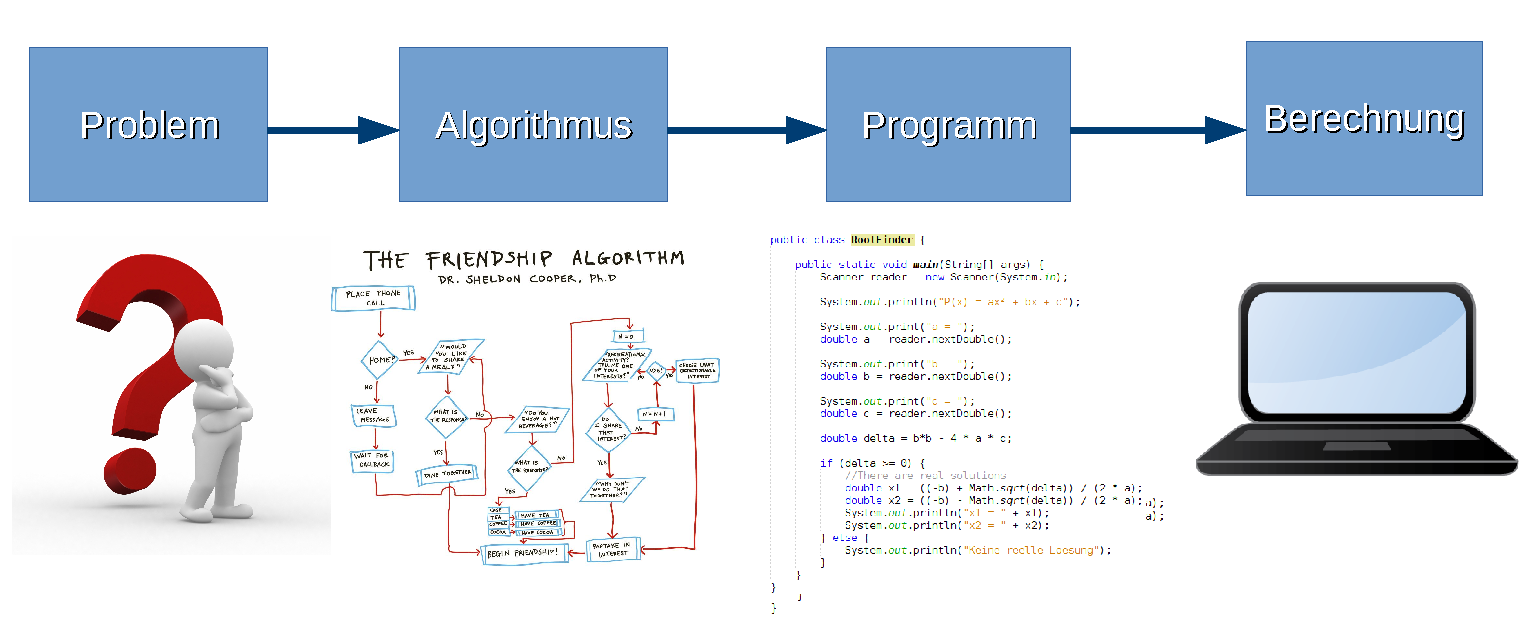
\includegraphics[width=\textwidth]{Alg-Prog-Schema}
	\end{frame}

	\begin{frame}
		\frametitle{Java ist eine Programmiersprache}
		\textit{\glqq Angefangen bei Laptops bis hin zu Rechenzentren, Spielekonsolen, wissenschaftlichen Supercomputern, Mobiltelefonen und dem Internet, Java wird überall verwendet.\grqq} \footnote{\url{https://www.java.com/de/about}}\\
		\pause
		\vspace{10pt}
		\begin{minipage}{.15\textwidth}
			
\includegraphics[width=\textwidth]{javalogo}
		\end{minipage}
		\begin{minipage}{.83\textwidth}
			\begin{itemize}
				\item 97\% aller Unternehmensdesktops nutzen Java
				\item 89\% aller Desktops (oder Rechner) in den USA nutzen Java
				\item 9 Millionen Java-Entwickler weltweit
				\item 3 Milliarden Mobiltelefone nutzen Java
				\item 100\% aller Blu-Ray-Player werden mit Java ausgeliefert
				\item ...
			\end{itemize}
		\end{minipage}
	\end{frame}

	\begin{frame}
		\frametitle{Programmiersprachen}
		\centering 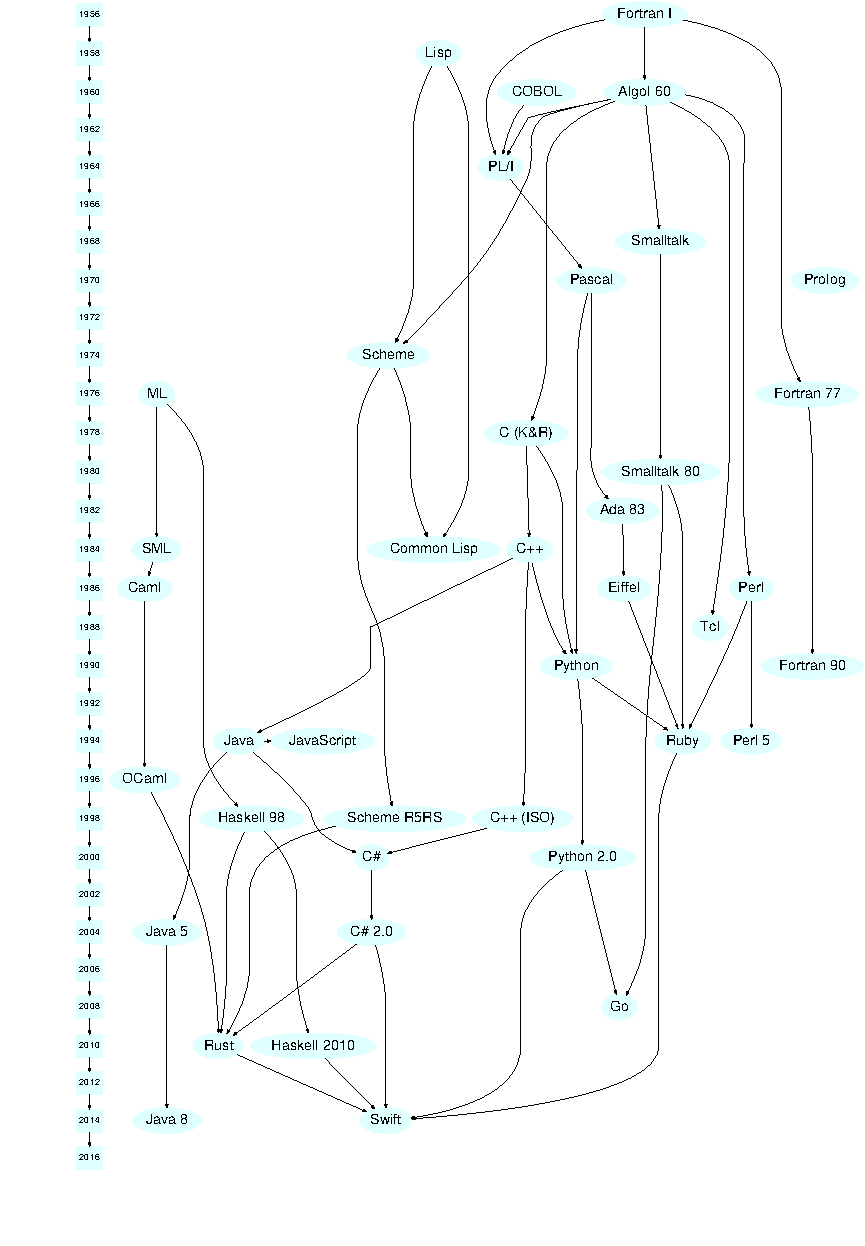
\includegraphics[height=.85\textheight]{Sprachen-Diagramm.pdf}
	\end{frame}

	%-------------------
	% Praxis
	%-------------------
	\section{Praxis}
	\begin{frame}
		\frametitle{Praxis}
		\tableofcontents[currentsection, currentsubsection] 
	\end{frame}

	\begin{frame}
		\frametitle{Compiler - NetBeans}
		\begin{itemize}
			\item Open JDK installieren
			\item \url{http://jdk.java.net}
			\item NetBeans herunterladen
			\item \url{https://netbeans.org} \\
			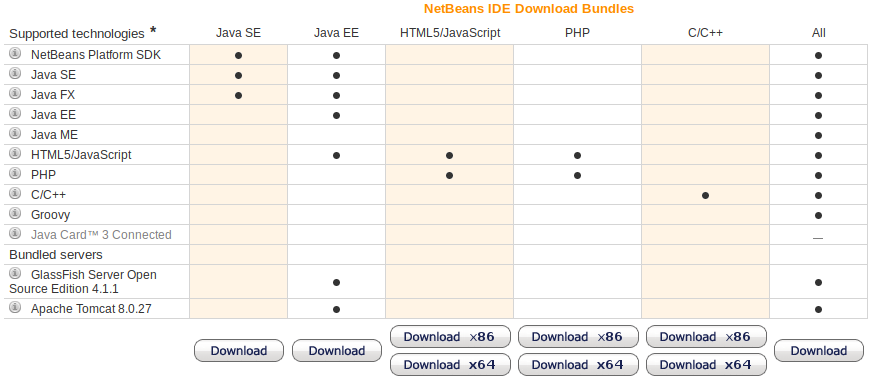
\includegraphics[width=.5\textwidth]{Netbeans-Download}
			\item Installieren
		\end{itemize}
	\end{frame}

	\begin{frame}
		\frametitle{Hello World}
		\begin{itemize}
			\item Ein neues Projekt erstellen: Java Application
			\item $System.out.println("Hello\ World!");$
			\pause
			\item $Scanner\ reader = new\ Scanner(System.in);$
			\item $reader.nextLine();$
			\pause
			\item $System.out.println("Bye\ World!");$
		\end{itemize}
	\end{frame}

	%-------------------
	% Zusammenfassung
	%-------------------
	\section{Zusammenfassung}
	\begin{frame}
		\frametitle{Zusammenfassung}
		\tableofcontents[currentsection, currentsubsection] 
	\end{frame}

	\begin{frame}
		\frametitle{Zusammenfassung}
		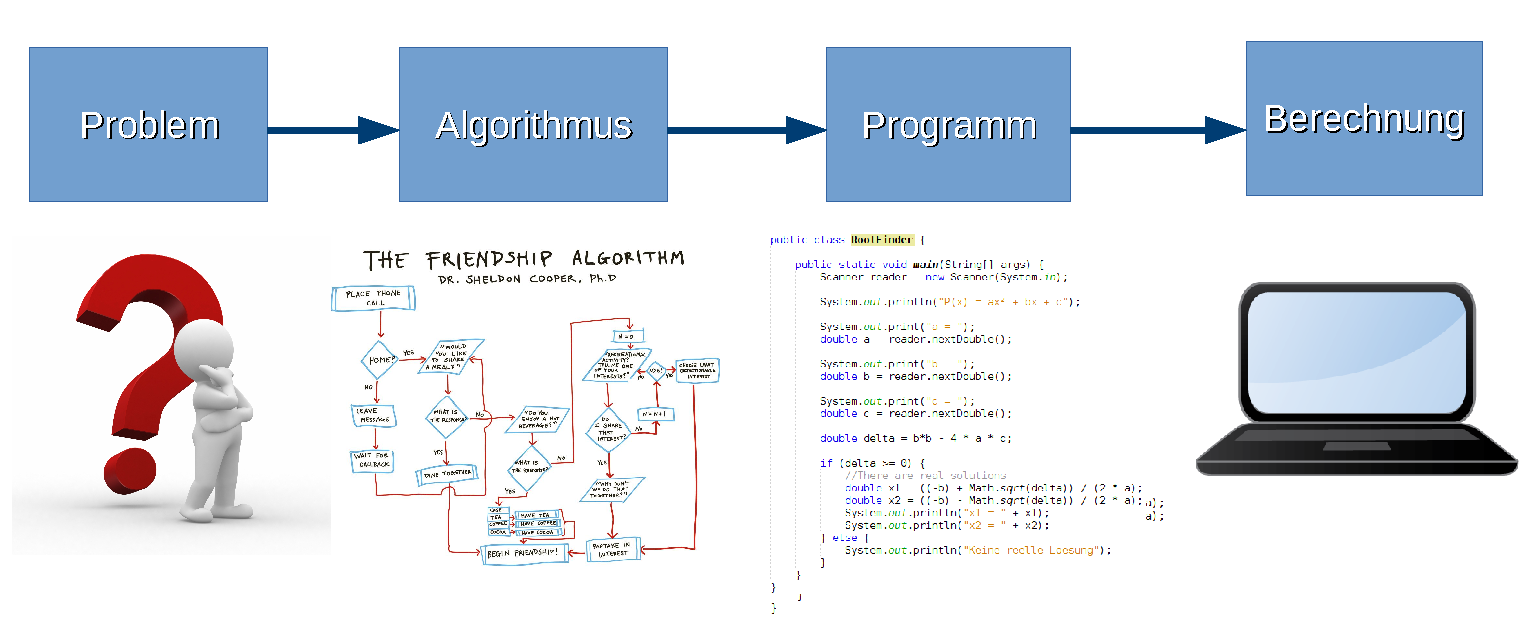
\includegraphics[width=\textwidth]{Alg-Prog-Schema}
		\begin{itemize}
			\item Nächste Woche: Variablen und Operatoren
		\end{itemize}
	\end{frame}

	\begin{frame}
		\frametitle{Literatur}
		\begin{itemize}
			\item Netbeans: \url{https://docs.oracle.com/javase/tutorial/getStarted/cupojava/netbeans.html}
			\item \url{https://edu.netbeans.org/contrib/slides/netbeans-platform}
			\item W3C Tutorial: 
			\begin{itemize}
				\item von: \url{https://www.w3schools.com/java/default.asp}
				\item bis: \url{https://www.w3schools.com/java/java\_comments.asp}
			\end{itemize}
			\item Exercises:
			\begin{itemize}
				\item Java Syntax: \url{https://www.w3schools.com/java/exercise.asp}
			\end{itemize}
		\end{itemize}
	\end{frame}

\end{document}
